%%%%%%%%%%%%%%%%%%%%%%%%%%%%%%%%%%%%%%%%%%%%%%%%%%%%%%%%%%%%%%%
% 音講論用スタイルファイル onkoron.sty の使用例
%
% 作成:2005年4月 9日 (初版)
%             4月15日 (Ver.1)
%             4月27日 (Ver.1.1)
%       2013年6月11日 (Ver.1.2)
%       2024年12月31日 (Ver.1.3) by Ryota NISHIMURA
%
%%%%%%%%%%%%%%%%%%%%%%%%%%%%%%%%%%%%%%%%%%%%%%%%%%%%%%%%%%%%%%%
%\documentclass[11pt,twocolumn]{jarticle} % 11pt(標準)
\documentclass[10pt,twocolumn]{jarticle} % 10pt(オプション)
\usepackage{onkoron}

%%%%%%%%%%%%%%%%%%%%%%%%%%%%%%%%%%%%%%%%%%%%%%%%%%%%%%%%%%%%%%%
% 参考文献の引用が [3,6,2,1] -> [1-3,6] になります.
\usepackage{cite}

%%%%%%%%%%%%%%%%%%%%%%%%%%%%%%%%%%%%%%%%%%%%%%%%%%%%%%%%%%%%%%%
% 行間を標準よりも広くしたい場合には,ここの数字を大きくして
% ください.逆に狭くしたい場合には,数字を小さくしてください.
\renewcommand{\baselinestretch}{1.0}

%%%%%%%%%%%%%%%%%%%%%%%%%%%%%%%%%%%%%%%%%%%%%%%%%%%%%%%%%%%%%%%
% 論文タイトルおよび脚注用の英文を記載する.
%
\title{日本音響学会講演論文集用スタイルファイル onkoron.sty の使い方
\thanks{How to use ``onkoron.sty'' to prepare a good-looking
manuscript for ASJ biannual meetings. by HARAZYUKU, Tar\^o, SHINJUKU,
Hanako (Saikyo Institute of Technology)}
}
%%%%%%%%%%%%%%%%%%%%%%%%%%%%%%%%%%%%%%%%%%%%%%%%%%%%%%%%%%%%%%%
% 講演者には○を付す.
% 講演者が粟屋潔学術奨励賞対象者の場合には◎を付す.
% 講演者が学生優秀発表賞対象者の場合には☆を付す.
% 連名の非会員には△を付す.
%
\author{◎原宿太郎, 新宿花子 (西工大)}
%
\begin{document}
\maketitle   

%--------------------------------------
\section{はじめに}
%--------------------------------------

本ファイルは,日本音響学会講演論文集(以下,音講論)用の原稿を TeX のス
タイルファイル onkoron.sty を用いて作成した例である。
文字サイズは 11 ptを標準とし,どうしても入りきらない場合には10 ptを使
用する。
以下,本ファイルに関する説明を本文中に記載した。
事前に本ファイルの中身を一読した上で使用することをお勧めする。

%--------------------------------------
\section{スタイルファイルの説明}
%--------------------------------------

%-----------------------------------------------------------------
\subsection{原稿のスタイルについて}
%-----------------------------------------------------------------

このスタイルファイルを用いて作成される原稿は,演題登録後に日本音響学会
から送付される「講演原稿の書き方」に基本的に沿ったものとなる。
タイトル,著者を1段組とし,本文は2段組として作成される。
タイトルの下に全著者名と各著者の所属を記載する。
ここで,著者の所属については,可能であれば略称で記載することが望ましい。
著者,所属記載後は,2段組で本文が始まる。
なお,1ページ目の一番下には脚注の欄として,タイトル,著者,所属の英語
訳を記載される。

%-----------------------------------------------------------------
\subsection{図表について}
%-----------------------------------------------------------------

図表のタイトルの挿入位置は,図は下,表は上である。
なお,図表は,天地にまとめるなどして,見易くすることを心掛ける。
この場合,Fig.~\ref{fig:thisfigure}のようになる。
また,大きい図表については,その部分のみ1段組として挿入する。
この場合には,
\begin{verbatim}
\begin{figure}[tb]
\end{verbatim}
に代えて,
\begin{verbatim}
\begin{figure*}[tb]
\end{verbatim}
を使用する。
この場合には,Fig.~\ref{fig:thatfigure}のようになる。
図とキャプションや,図と本文の間隔を微調整したい時には,\verb|\vspace|
が使用できる。

%
\begin{figure}[tb]
\begin{center}
%\vspace{-10pt}   % 本文と図の間隔微調整用
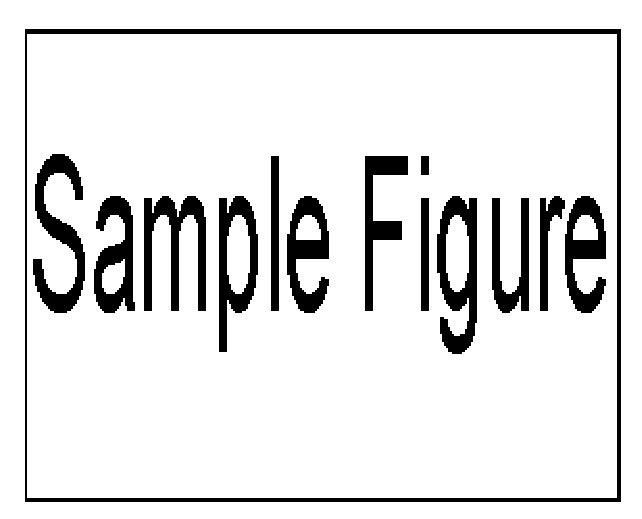
\includegraphics[width=0.8\columnwidth]{sample.eps}
\vspace{-10pt}     % 図とキャプションの間隔微調整用
\end{center}
\caption{Caption of this figure}
\label{fig:thisfigure}
%\vspace{-10pt}   % キャプションと本文の間隔微調整用
\end{figure}
%
%
\begin{table}
%\vspace{-10pt}   % 本文とキャプションの間隔微調整用
\caption{Caption of this table}
\label{tbl:thistable}
\begin{center}
%\vspace{-10pt}   % キャプションと表の間隔微調整用
\begin{tabular}{|l|lll|}\hline
& a & b & c\\\hline
$\alpha$ & 1 & 2 & 3\\
$\beta$ & 4 & 5 & 6\\
$\gamma$ & 7 & 8 & 9\\\hline
\end{tabular}
\vspace{-10pt}   % 表と本文の間隔微調整用
\end{center}
\end{table}
%
%
\begin{figure*}[tb]
\begin{center}
%\vspace{-10pt}   % 本文と図の間隔微調整用
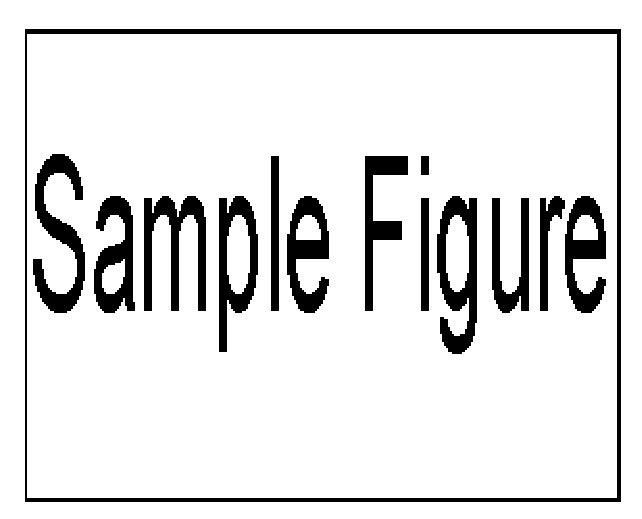
\includegraphics[width=0.8\columnwidth]{sample.eps}
\vspace{-10pt}     % 図とキャプションの間隔微調整用
\end{center}
\caption{Caption of this figure}
\label{fig:thatfigure}
%\vspace{-10pt}   % キャプションと本文の間隔微調整用
\end{figure*}
%
%-----------------------------------------------------------------
\subsection{本文について}
%-----------------------------------------------------------------

本文の表記については,日本音響学会誌の投稿規定に準拠して記載する。
本文中で参考文献を引用する際は,引用箇所に番号を記載する。
その際には,$^{[1]}$のように番号を括弧で囲んで上付で挿入するか,文献
[1]のように表記する。
$^{[1]}$のように記載したい場合には,onkoron.sty 中にある
\begin{verbatim}
%\def\@cite#1#2{$^{\hbox{\scriptsize \
          {[#1\if@tempswa , #2\fi}]}}$}
\end{verbatim}
の行のコメントを外せばよい。
同一箇所に複数の参考文献を引用する際は,\cite{article,sansho},
\cite{article,book,taka,sato}のように,まとめて記載する。
さらに,同一番号で参考文献欄に書誌情報を記載する。
その他については,標準的な方法に習って書き表す\cite{sansho}。

%-----------------------------------------------------------------
\subsection{謝辞について}
%-----------------------------------------------------------------

必要に応じて,本文の最後,参考文献の前に謝辞を挿入する。
また,謝辞は節ではなく,
\begin{verb}
\paragraph{謝辞}
\end{verb}
で書くようにする。

%-----------------------------------------------------------------
\subsection{参考文献について}
%-----------------------------------------------------------------

参考文献自体のフォントサイズは本文と同様である。
少なくとも,正しく引用するのに必要な情報は記載する。
著者が3名以上いる場合は,第一著者のみ記載し,「他」,「{\itshape et
al.}」を入れる。
書誌情報のフォーマットの例は,本ファイルの最後の「参考文献」欄に記載し
てあるので,参照されたい。

%-----------------------------------------------------------------
\subsection{bibtexについて}
%-----------------------------------------------------------------

LLMに.bstを作成させました。とりあえず動く版ということで,利用は自己責任でお願いします。よりスッキリ実装させたり,問題を発見したりした場合には,github\footnote{\url{https://github.com/tokudai-nishimura-lab/genkou-kit\_utf-8\_plus\_bst}}のissueに書くか,pullリクエストしていただけると非常に嬉しいです.

複数文献を一つのcite内で引用した場合に,全部の数字が羅列されずに省略されるテスト\cite{obashi19ASJ,Dia_system,setoAPSIPA2018}。

%-----------------------------------------------------------------
\section{その他のTIPS}
%-----------------------------------------------------------------

以下に,TeX を使って見やすい原稿を作成するための,TIPSを参考までに示す。
\begin{itemize}
\itemsep -5pt
\item 本文中に,周波数 1000 Hz,音圧レベル 40~dB といった値を記載する
際は,数値と単位の間に半角スペースを入れる。
ただし,{}「C$^\circ$」と「\%」の場合には,スペースを入れずに記す。
\item 図番号をFig.\verb|\ref{fig:thisfigure}|として本文で参照すると,
これが行末に来た場合に,Fig.と図番号の間で改行されてしまうことがある。
これを防ぐためには,Fig.\verb|~\ref{fig:thisfigure}|とする。
\item 「,」と「「」が並ぶと,その間隔が狭くなる。この場合,{}「,\{\}
「」と記すとよい。
\item \textit{et al.}は斜体なので,\verb|{\itshape et al.}|とするか,
\verb|\textit{et al.}|とする。
\item 式(\verb|\ref{eqn:thisequation}|)に代えて,式
\verb|\eqref{eqn:thisequation}|を用いることもできる。
\item サンプルのソースコード上に書かれている,\verb,\verb|  |,は,TeX
のコマンド文字列を,ただの文字列として表示させるためのものである。
\item dvipdf で PDF ファイルを作成した時に文章位置が狂う場合には,
{\tt -sPAPERSIZE=a4} のオプションを付けて実行してみる。
\item dvipdfmx で PDF ファイルを作成すると,フォントを埋め込まないので,ファイルサイズを小さくできる。
\end{itemize}

%-----------------------------------------------------------------
\section{おわりに}
%-----------------------------------------------------------------

本稿が,分かりやすい原稿づくりの参考になれば,幸いである。

%-----------------------------------------------------------------
\paragraph{謝辞}
%-----------------------------------------------------------------

脚注を段抜きにするために,Bear-Collections \cite{bear}
にある 1-in-2.sty の該当箇所を,アレンジして本スタイルファイルに取り込
ませていただきました。

%-----------------------------------------------------------------
% 参考文献
%-----------------------------------------------------------------

\bibliographystyle{onkoron}
\bibliography{myrefs}

% \begin{thebibliography}{9} % 参考文献が10以上ある場合は{99}とする
% \itemsep -5pt             % 項目の間隔微調整用
% \bibitem{article}
% 著者名,雑誌名,巻(号),ページ,年.
% \bibitem{book}
% 著者名,``文献名,'' 出版社名,年.
% \bibitem{taka}
% 高橋,鈴木,音講論(春),123-124,2005.
% \bibitem{sato}
% Sato {\itshape et al.}, Acoust. Sci. Tech., 1 (2), 34-45, 2005.
% \bibitem{sansho}
% 三省堂編修所編,``新しい国語表記ハンドブック,'' 三省堂,1991.
% \bibitem{bear}
% http://mechanics.civil.tohoku.ac.jp/\verb|~|bear/\\bear-collections/index-j.html
% \end{thebibliography}

\end{document}
